\cotefile{148}
\scanpage{18}

$4$ sommets d'ordre $6$ $+\unsure{6}$ sommets d'ordre $6$ $+12$ sommets d'ordre $3$

$24$ triangles $+4$ hexagones

% D1: upper-left pencil drawing; listing-paper stripes are not drawing strokes.
\figure{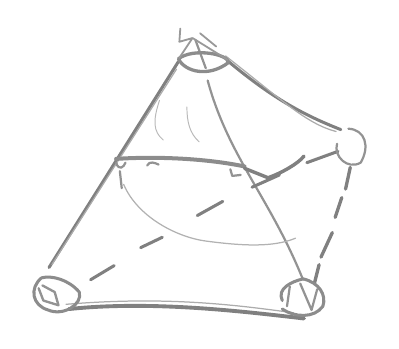
\begin{tikzpicture}[x=0.012cm,y=-0.012cm,line cap=round,line join=round]
\draw[gray,line width=1.1pt] (45,268)--(182,50) (234,49)..controls(283,90)and(316,107)..(354,122);
\draw[gray,line width=1.4pt] (66,312)..controls(153,303)and(246,314)..(315,322);
\draw[gray!65,line width=.45pt] (48,265)--(180,58) (232,44)..controls(292,91)and(318,116)..(349,124) (63,307)..controls(171,298)and(245,308)..(304,316);
\draw[gray!85,line width=.8pt] (200,27)--(211,57) (213,70)..controls(235,151)and(279,194)..(314,281);
\draw[gray,line width=1.2pt] (364,162)--(359,185) (355,194)--(348,215) (345,231)--(333,257) (331,265)--(326,285);
\draw[gray,line width=1.1pt] (89,281)--(114,266) (142,247)--(165,236) (202,213)--(229,198) (260,183)--(289,170) (318,157)--(351,145);
\draw[gray!90,line width=1.2pt] (182,47)..controls(189,61)and(214,67)..(235,51)..controls(235,42)and(198,35)..(182,47);
\draw[gray!80,line width=.65pt] (183,46)--(197,25)--(234,48) (205,20)--(222,34) (184,15)--(183,29)--(197,25);
\draw[gray!90,line width=1.1pt] (37,279)..controls(24,290)and(27,308)..(44,313)..controls(60,320)and(81,307)..(77,294)..controls(66,281)and(48,276)..(37,279);
\draw[gray!85,line width=.85pt] (38,287)--(51,294)--(55,308)--(39,303)--(34,290);
\draw[gray!90,line width=1.1pt] (292,303)..controls(286,290)and(302,283)..(314,280)..controls(331,284)and(339,297)..(335,309)..controls(326,322)and(305,321)..(292,312);
\draw[gray!85,line width=.8pt] (311,285)--(323,313)--(329,291) (300,288)--(297,309);
\draw[gray!85,line width=.8pt] (362,121)..controls(380,122)and(385,140)..(375,157)..controls(361,165)and(346,150)..(350,137);
\draw[gray!90,line width=1.45pt] (116,153)..controls(162,150)and(214,153)..(252,161);
\draw[gray!85,line width=.8pt] (116,157)..controls(119,166)and(124,162)..(126,157) (120,166)--(122,184) (149,160)..controls(151,155)and(157,157)..(161,159) (237,164)--(239,171)--(248,170);
\draw[gray,line width=1.25pt] (252,163)--(277,173)..controls(291,168)and(309,158)..(315,150);
\draw[gray!60,line width=.45pt] (124,180)..controls(139,215)and(181,236)..(211,240)..controls(249,245)and(282,247)..(306,237);
\draw[gray!55,line width=.35pt] (162,91)..controls(155,112)and(155,124)..(166,133) (191,98)..controls(191,114)and(194,126)..(204,135);
\end{tikzpicture}}

% D2: upper-right drawing, with six black interior marks and five red junctions.
\figure{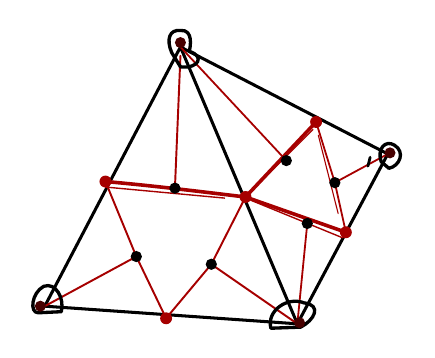
\begin{tikzpicture}[x=0.014cm,y=-0.014cm,line cap=round,line join=round]
\draw[line width=1.1pt] (28,259)--(151,24)--(339,121)--(257,275)--cycle (151,24)--(257,275);
\draw[red!65!black,line width=1.3pt] (83,146)..controls(129,150)and(176,156)..(210,160)--(301,192) (210,160)--(274,92);
\draw[red!65!black,line width=.5pt] (83,151)--(191,161) (215,163)--(298,197) (213,157)--(271,99);
\draw[red!65!black,line width=.7pt] (151,32)--(146,152) (83,146)--(111,214)--(138,270)--(179,221)--(210,160) (28,259)--(111,214) (257,275)--(179,221);
\draw[red!65!black,line width=.65pt] (151,24)--(247,127) (274,92)--(291,147)--(301,192) (339,121)--(291,147) (257,275)--(266,184);
\draw[red!65!black,line width=.4pt] (276,104)--(294,175);
\foreach \p in {(83,146),(210,160),(301,192),(138,270),(274,92)}{\fill[red!65!black] \p circle (5.4);}
\foreach \p in {(146,152),(111,214),(179,221),(247,127),(291,147),(266,184)}{\fill \p circle (5.1);}
\draw[line width=1pt] (321,132)--(323,124);
\draw[line width=1.2pt] (22,265)..controls(14,265)and(16,247)..(27,241)..controls(38,237)and(46,252)..(43,264)--cycle;
\draw[line width=1.2pt] (143,29)..controls(138,17)and(141,8)..(151,9)..controls(163,8)and(160,24)..(159,28)..controls(173,32)and(168,44)..(151,42)--(143,29);
\draw[line width=1.2pt] (233,279)..controls(229,263)and(248,250)..(263,256)..controls(280,258)and(272,272)..(260,278)--cycle;
\draw[line width=1.2pt] (333,128)..controls(329,116)and(337,108)..(345,113)..controls(355,119)and(350,132)..(340,134)--cycle;
\foreach \p in {(24,259),(151,20),(259,274),(341,120)}{\fill[red!28!black] \p circle (5);}
\end{tikzpicture}}

\margin{mieux\par cf verso\par (subdivision\par barycentrique)}

\[
\begin{aligned}
s_0&=4+6+\unsure{4}.3=22\\
s_1&=12+4.\unsure{9|8}=\unsure{48}\\
s_2&=4.7=28
\end{aligned}
\]

% D3: upper sphere, irregular small contours and actual separated point marks.
\figure{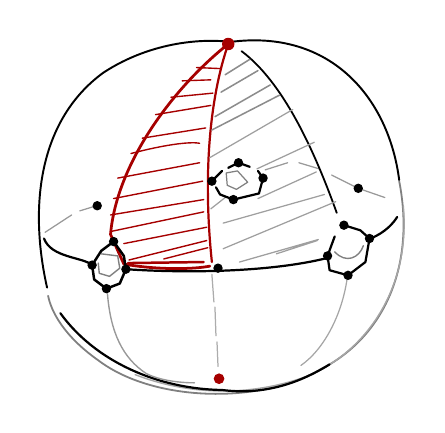
\begin{tikzpicture}[x=0.013cm,y=-0.013cm,line cap=round,line join=round]
\draw[line width=.7pt] (33,261)..controls(15,181)and(25,97)..(88,51)..controls(137,19)and(189,18)..(212,21)..controls(311,8)and(367,77)..(377,156);
\draw[gray,line width=.65pt] (377,157)..controls(393,239)and(363,309)..(300,341)..controls(241,375)and(137,373)..(83,332)..controls(49,308)and(37,284)..(34,269);
\draw[gray!70,line width=.5pt] (381,181)..controls(389,268)and(337,331)..(280,350)..controls(225,368)and(168,365)..(119,346);
\draw[line width=.8pt] (46,286)..controls(80,333)and(141,360)..(204,361)..controls(251,367)and(286,350)..(309,336);
\draw[line width=.8pt] (30,213)..controls(37,232)and(68,231)..(77,239) (110,243)..controls(169,247)and(251,246)..(307,232) (349,213)..controls(364,207)and(372,197)..(375,192);
\draw[gray!80,line width=.45pt] (31,207)--(57,190) (65,186)--(78,182) (246,146)--(268,139) (279,139)--(299,145) (311,151)--(337,164)--(363,173);
\draw[red!65!black,line width=1pt] (210,23)..controls(157,65)and(101,139)..(95,209)--(108,238)..controls(142,244)and(177,243)..(192,240);
\draw[red!65!black,line width=.8pt] (210,23)..controls(192,75)and(185,150)..(194,236);
\draw[line width=.65pt] (223,30)..controls(263,60)and(293,124)..(316,188);
\draw[gray!70,line width=.45pt] (326,253)..controls(321,287)and(304,321)..(281,337);
\draw[gray!80,line width=.5pt] (92,267)..controls(95,305)and(107,330)..(130,345)..controls(144,352)and(164,354)..(177,354);
\draw[gray!65,line width=.45pt] (194,248)--(196,275) (197,280)--(198,308) (199,314)--(200,338);
\draw[red!65!black,line width=.5pt] (179,46)--(202,47) (165,59)--(193,58) (154,75)--(195,71) (139,92)--(193,83) (126,115)--(188,105) (115,130)..controls(145,122)and(172,118)..(182,120) (102,154)--(182,139) (98,174)--(185,157) (95,190)--(186,175) (96,206)--(186,187) (108,218)--(189,202) (113,234)--(189,215) (147,233)--(190,222);
\draw[red!65!black,line width=.9pt] (112,237)--(186,236);
\draw[gray!90,line width=.55pt] (207,53)--(231,38) (203,70)--(239,49) (197,94)--(251,63) (194,107)--(260,73);
\draw[gray!75,line width=.45pt] (192,134)--(273,87) (238,145)--(294,119) (193,184)--(207,173) (239,174)--(296,148) (205,198)--(304,170) (205,223)--(315,177) (221,236)--(298,214) (257,228)--(297,215);
\draw[line width=.9pt] (98,216)--(108,230)--(110,243)--(104,257)--(91,262)--(79,253)--(77,239)--(86,225)--(98,216);
\draw[gray,line width=.5pt] (86,228)--(102,230)--(104,242)--(94,250)--(84,247)--(83,237);
\draw[line width=.8pt] (194,157)--(204,147) (210,144)--(220,139)--(231,143) (239,147)--(244,154)--(240,169)--(215,175)--(202,170)--(198,163);
\draw[gray,line width=.45pt] (208,149)--(219,147)--(229,158)--(218,165)--(209,161)--cycle;
\draw[line width=.8pt] (323,200)--(339,205)--(348,213)--(344,236)--(327,249)--(309,244)--(307,230)--(314,211);
\draw[gray,line width=.5pt] (314,226)..controls(325,238)and(338,232)..(342,220);
\foreach \p in {(98,216),(110,243),(91,262),(77,239),(194,157),(220,139),(244,154),(215,175),(323,200),(348,213),(327,249),(307,230),(82,181),(200,242),(337,164)}{\fill \p circle (4.6);}
\fill[red!65!black] (210,23) circle (6.1);
\fill[red!65!black] (201,350) circle (5.2);
\end{tikzpicture}}

% D4: central coloured tetrahedron. The lower oblique connector begins above
% the t of the following heading; its terminal return is drawn without an idealized head.
\figure{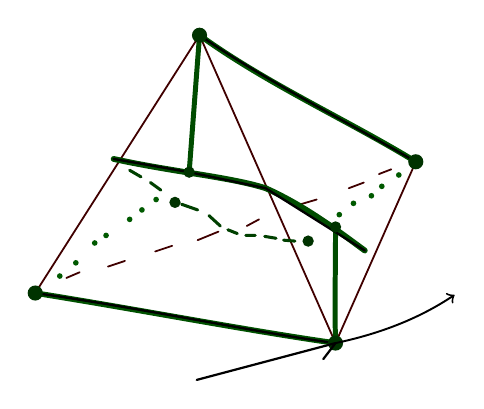
\begin{tikzpicture}[x=0.012cm,y=-0.012cm,line cap=round,line join=round]
\draw[red!25!black,line width=.65pt] (36,304)--(210,31)--(354,357)--(439,165);
\draw[green!32!black,line width=2pt] (36,304)..controls(143,321)and(262,344)..(354,357) (210,31)..controls(282,83)and(369,122)..(439,165);
\draw[line width=.85pt] (36,304)..controls(150,320)and(276,347)..(354,357) (210,31)..controls(280,79)and(365,122)..(439,165);
\draw[red!25!black,line width=.65pt] (69,288)--(83,282) (113,276)--(131,270) (163,260)--(181,254) (208,248)--(230,239) (260,233)--(273,226) (317,210)--(334,205) (368,193)--(384,187) (400,178)--(413,173);
\draw[green!30!black,line width=2.1pt] (119,162)..controls(183,176)and(242,181)..(280,193)..controls(323,212)and(363,243)..(385,259);
\draw[green!30!black,line width=1.8pt] (210,31)--(199,176) (354,234)..controls(354,278)and(353,318)..(354,357);
\draw[line width=.85pt] (119,162)--(199,176)--(280,193)--(385,259);
\draw[green!25!black,line width=1.1pt] (136,174)--(148,181) (158,187)--(169,195) (191,210)--(208,216) (220,222)--(232,233) (240,237)--(250,241) (259,243)--(269,243) (279,244)--(291,246) (299,248)--(311,249);
\foreach \p in {(62,286),(79,272),(99,251),(111,243),(136,226),(149,216),(164,205),(358,221),(373,209),(392,201),(403,191),(421,179)}{\fill[green!35!black] \p circle (3);}
\foreach \p in {(184,208),(325,249),(199,176),(354,234)}{\fill[green!20!black] \p circle (6);}
\foreach \p in {(36,304),(210,31),(354,357),(439,165)}{\fill[green!20!black] \p circle (8);}
\draw[->,line width=.7pt] (354,357)..controls(411,345)and(450,326)..(480,306);
\draw[line width=.8pt] (207,396)--(354,357)--(341,374);
\end{tikzpicture}}

\margin{ça fait $2^{\unsure{9|4}}-1=15$\par possibilités \unsure{inversion|limites}\par des faces choisies\par \unsure{en} \illegible{2} \unsure{de}\par vue !}

\uline{$4$ types de points-base}

$\bullet$ $3$ structures carrées sur $I$ (ou $J$)

$\textcolor{red!70!black}{\bullet}$ $2$ structures tétraédrales $=$ \unsure{orientation|orientations}\margin{des faces}

$\textcolor{red!30!black}{\bullet}$ $6$ structures \inserted{bi}pantaloniques\margin{opposées}\par
\hspace*{1em}(maillot ceinturé)\par
\hspace*{1em}(carrée $+$ codiagonale) $\simeq$\par
\hspace*{3em}repère de $J$)

\[
\updownarrow
\]

$\bullet$ $6$ structures pantaloniques\par
\hspace*{3em}de guingois\par
\hspace*{1em}(quart de tour)\par
(\unsure{$\simeq|=$} carré, $+$ orientation de $I$ i.e.)\par
\hspace*{4em}de $J$ $\simeq$ repère de $J$)

% F1: the raised looped glyph is preserved graphically; its alphabetic/numeric identity is open.
\margin{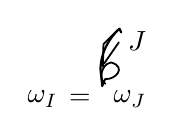
\begin{tikzpicture}[x=.75cm,y=.75cm,line cap=round,line join=round,baseline=(wI.base)]
\node[inner sep=0pt] (wI) at (0,0) {$\omega_I$};
\node[inner sep=0pt] at (.63,0) {$=$};
\node[inner sep=0pt] at (1.48,0) {$\omega_J$};
\draw[line width=.8pt] (1.01,.22)--(.98,.50)..controls(.98,.78)and(1.13,1.04)..(1.30,1.19)--(1.33,1.13);
\draw[line width=.65pt] (1.06,.26)..controls(.95,.32)and(.98,.59)..(1.16,.62)..controls(1.43,.54)and(1.23,.32)..(1.06,.34)--(1.01,.22);
\draw[line width=.65pt] (1.04,.60)--(1.29,.96) (1.02,.55)--(1.03,.93)--(1.27,1.17);
\node[inner sep=0pt] at (1.60,.99) {$J$};
\node[inner sep=0pt] at (1.86,.63) {$\unsure{\phantom{A}}$};
\end{tikzpicture}}

\diagram{\begin{tikzcd}[ampersand replacement=\&]
\operatorname{rep}(J) \arrow[d,leftrightarrow]\\
J\times\omega_J
\end{tikzcd}}

% D5: lower small sphere; the central open double-bowed contour is drawing ink.
\figure{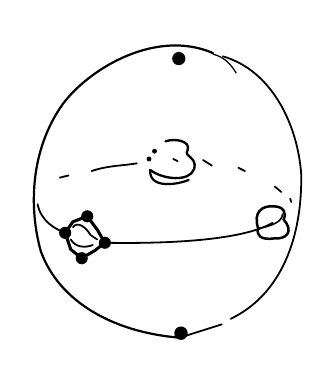
\begin{tikzpicture}[x=.014cm,y=-.014cm,line cap=round,line join=round]
\draw[line width=.8pt] (179,21)..controls(128,-1)and(68,34)..(43,67)..controls(13,109)and(12,162)..(23,201)..controls(40,247)and(89,274)..(148,279);
\draw[line width=.65pt] (188,24)..controls(233,37)and(256,87)..(259,131)..controls(260,188)and(241,240)..(195,262) (187,267)--(149,279);
\draw[line width=.45pt] (179,22)..controls(190,25)and(195,31)..(200,39);
\draw[line width=.65pt] (20,158)..controls(23,174)and(37,181)..(45,184) (81,193)..controls(138,194)and(205,191)..(233,175);
\draw[line width=.65pt] (40,134)--(48,132) (69,128)..controls(83,123)and(99,123)..(110,121) (170,118)--(178,123) (202,125)--(208,128) (235,142)--(241,147) (249,153)--(250,156);
\fill (121,117) circle (2.2); \fill (126,110) circle (2.2);
\draw[line width=.65pt] (143,117)--(147,119);
\draw[line width=.85pt] (136,101)..controls(145,98)and(159,101)..(156,109)..controls(152,115)and(165,115)..(162,126)..controls(158,138)and(134,136)..(122,127);
\draw[line width=.8pt] (122,127)..controls(121,145)and(148,140)..(157,136);
\draw[line width=1.1pt] (45,184)--(52,174)--(65,169)--(74,181)--(81,193)--(72,200)--(60,207)--(50,199)--cycle;
\draw[line width=.65pt] (52,179)..controls(56,173)and(64,179)..(68,186)--(74,190) (50,190)..controls(54,197)and(63,198)..(70,195);
\foreach \p in {(45,184),(65,169),(81,193),(60,207)}{\fill \p circle (5.5);}
\draw[line width=.9pt] (220,180)..controls(215,165)and(224,159)..(234,160)..controls(243,160)and(246,166)..(243,172)..controls(253,183)and(245,190)..(235,189)..controls(222,191)and(218,186)..(220,180);
\draw[line width=.55pt] (220,180)..controls(232,178)and(242,174)..(242,167);
\fill (148,26) circle (6); \fill (150,275) circle (6.1);
\end{tikzpicture}}

% D6: four-holed small drawing; open upper contours and unequal central strokes.
\figure{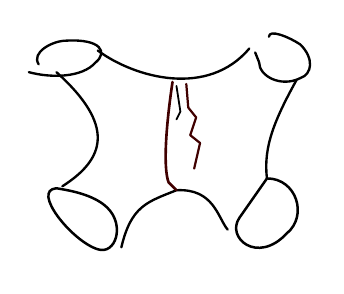
\begin{tikzpicture}[x=.025cm,y=-.025cm,line cap=round,line join=round]
\draw[line width=.85pt] (52,23)..controls(71,37)and(108,47)..(129,22) (31,34)..controls(61,61)and(56,78)..(34,92) (153,38)..controls(142,58)and(136,72)..(138,88) (64,123)..controls(69,102)and(77,100)..(92,94)..controls(111,93)and(113,108)..(118,114);
\draw[line width=.85pt] (22,30)..controls(18,24)and(29,18)..(36,18)..controls(54,17)and(57,24)..(51,29)..controls(44,37)and(28,37)..(17,34);
\draw[line width=.85pt] (139,16)..controls(139,12)and(149,16)..(155,20)..controls(162,27)and(161,35)..(155,37)..controls(145,42)and(134,36)..(134,29)--(132,24);
\draw[line width=.9pt] (31,93)..controls(18,94)and(39,120)..(52,124)..controls(61,127)and(66,112)..(57,103)..controls(50,96)and(37,94)..(31,93);
\draw[line width=.9pt] (138,88)..controls(153,88)and(159,107)..(148,116)..controls(133,132)and(117,118)..(124,108)--(138,88);
\draw[red!25!black,line width=.95pt] (90,39)..controls(87,59)and(85,82)..(88,90)--(92,94);
\draw[red!25!black,line width=.8pt] (97,40)--(98,52)--(102,57)--(99,66)--(104,70)--(101,83);
\draw[line width=.65pt] (92,41)--(94,54)--(92,58);
\end{tikzpicture}}

\margin{sur cette figure, on\par voit à la fois la \unsure{p.r.q.|proj.}\par du tétraèdre à la\par configuration-carré,\par et à la configuration\par bien pantalonique\par du guin-gois.}

% D7: lower large truncated drawing; the short corner tips and bowed trace are pencil.
\figure{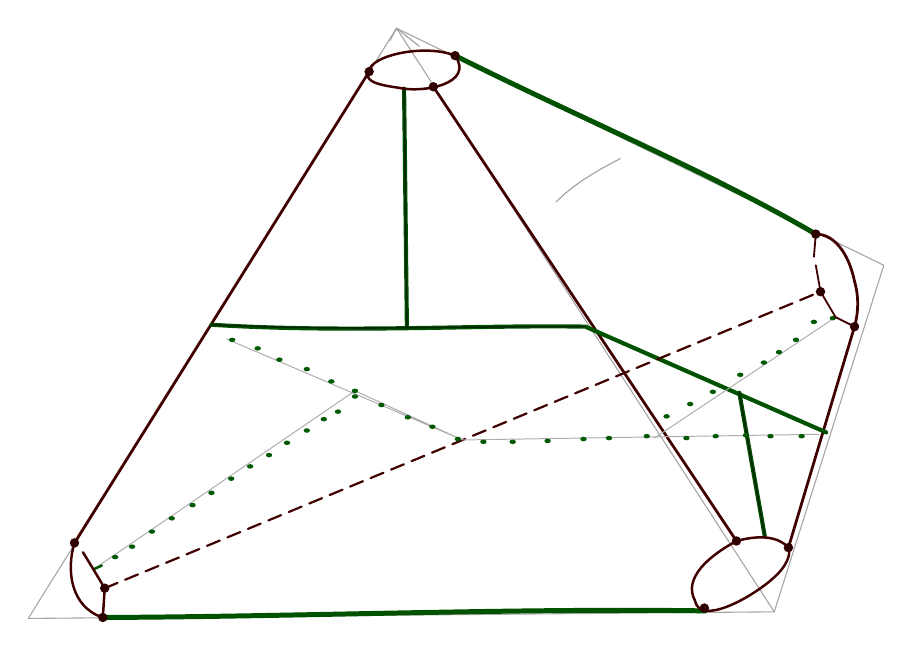
\begin{tikzpicture}[x=.012cm,y=-.012cm,line cap=round,line join=round]
\draw[gray!70,line width=.4pt] (20,642)--(410,17)--(926,268)--(810,635)--cycle (410,17)--(810,635);
\draw[gray!75,line width=.4pt] (403,30)--(410,17)--(434,36) (579,201)..controls(599,181)and(622,168)..(647,155);
\draw[red!25!black,line width=1pt] (69,562)--(381,63) (449,79)--(770,560) (825,567)--(895,333);
\draw[green!32!black,line width=1.8pt] (472,46)..controls(612,116)and(737,167)..(854,235) (99,641)..controls(313,640)and(539,631)..(737,634);
\draw[green!32!black,line width=1.5pt] (214,331)..controls(362,340)and(491,331)..(610,333)--(865,445) (418,81)--(421,334) (773,403)--(800,555);
\draw[green!15!black,line width=.55pt] (214,331)..controls(362,338)and(491,332)..(610,333) (418,81)--(421,334) (773,403)--(800,555);
\draw[red!25!black,dash pattern=on 5pt off 3pt,line width=.8pt] (101,610)--(859,296);
\draw[gray!65,line width=.35pt] (89,590)--(366,401)--(480,453)--(857,447) (230,346)--(480,453) (683,451)--(875,323);
\foreach \p in {(112,577),(130,566),(151,550),(172,536),(194,522),(214,509),(235,494),(255,481),(275,469),(294,456),(315,443),(333,431),(348,423),(366,407),(236,347),(263,356),(286,368),(315,378),(341,391),(366,401),(394,416),(422,429),(448,439),(475,452),(502,455),(533,455),(570,454),(608,452),(635,451),(675,449),(717,451),(748,449),(780,448),(806,449),(839,449),(696,428),(721,415),(745,402),(774,384),(799,371),(815,360),(833,347),(852,328),(872,324)}{\fill[green!35!black] \p ellipse (3.4 and 2.4);}
\draw[green!35!black,line width=.9pt] (89,590)--(98,586);
\draw[red!25!black,line width=.9pt] (381,63)..controls(381,46)and(440,33)..(472,46)..controls(493,76)and(438,86)..(412,80)..controls(390,77)and(375,73)..(381,63);
\draw[red!25!black,line width=.9pt] (69,562)..controls(60,591)and(65,630)..(99,641) (99,641)--(101,610)--(89,590)--(78,572);
\draw[red!25!black,line width=1pt] (854,235)..controls(874,235)and(889,256)..(895,285)..controls(902,309)and(896,329)..(895,333);
\draw[red!25!black,line width=.65pt] (854,235)--(852,259) (854,268)--(859,296)--(875,323)--(895,333);
\draw[red!25!black,line width=.9pt] (770,560)..controls(742,575)and(713,599)..(726,623)..controls(731,650)and(784,621)..(807,601)..controls(824,587)and(828,573)..(825,567)..controls(813,554)and(792,554)..(770,560);
\foreach \p in {(69,562),(101,610),(99,641),(381,63),(472,46),(449,79),(770,560),(825,567),(736,631),(854,235),(859,296),(895,333)}{\fill[red!18!black] \p circle (5);}
\end{tikzpicture}}

$4$ \uline{types de chemins élémentaires}$^{*}$

a) ``quart de twist'' $(2\times3\times4\unsure{)}$\par
\hspace*{2em}(contour d'un trou)

b) ``sixième de tour'' $(2\times2\times3)$\par
\hspace*{2em}(sur équateur)

c) pôle vers trou $(2\times2\times3)$\par
\hspace*{2em}et inv.

d) pôle vers équateur\par
\hspace*{2em}et inv. $(2\times2\times3)$

$2$ types composés supplém.

e) trou vers trou $(2\times3)$\par
\hspace*{2em}ou ``tiers de tour''

f) demi twist $(2\times2\times3)$

[et bien sûr, g) twist complet $2\times2\times3)$]

\uline{relations} ...

% D8: bottom sphere; rear equatorial arrow ends before the rear-left point.
\figure{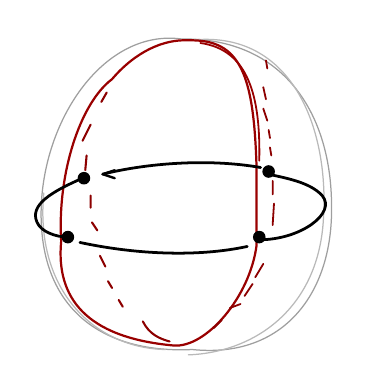
\begin{tikzpicture}[x=.017cm,y=-.017cm,line cap=round,line join=round]
\draw[gray!75,line width=.45pt] (129,18)..controls(70,10)and(23,81)..(24,151)..controls(25,222)and(72,253)..(137,250)..controls(205,257)and(242,208)..(241,143)..controls(241,76)and(207,17)..(129,18);
\draw[gray!55,line width=.45pt] (135,19)..controls(211,10)and(239,84)..(235,151)..controls(232,218)and(185,252)..(134,254) (26,133)..controls(19,207)and(65,249)..(117,250);
\draw[red!60!black,line width=.8pt] (134,19)..controls(173,18)and(183,44)..(185,115)--(185,172)..controls(180,211)and(147,249)..(123,247)..controls(57,241)and(35,211)..(39,169)..controls(36,119)and(53,66)..(77,48)..controls(94,28)and(115,18)..(134,19);
\draw[red!60!black,line width=.65pt] (143,21)..controls(179,26)and(188,61)..(187,109);
\draw[red!55!black,line width=.75pt] (73,58)--(69,65) (61,82)--(55,94) (58,105)--(57,116) (61,135)--(61,144) (62,155)--(66,161) (68,180)--(72,188) (74,199)--(77,204) (82,213)--(85,218) (100,229)..controls(105,239)and(113,242)..(120,244);
\draw[red!55!black,line width=.65pt] (192,34)--(193,40) (190,54)--(192,63) (190,70)--(193,79) (194,86)--(195,92) (195,99)--(196,105) (197,124)--(197,134) (198,141)--(197,157) (190,186)--(184,196) (182,201)--(176,210) (173,216)--(165,219) (159,228)--(153,234);
\draw[line width=1pt] (55,122)..controls(32,132)and(15,142)..(21,155)..controls(24,162)and(35,166)..(44,166) (53,170)..controls(95,179)and(141,181)..(178,173) (187,168)..controls(218,168)and(245,148)..(234,135)..controls(225,125)and(207,122)..(194,119);
\draw[line width=1pt] (188,114)..controls(148,107)and(102,111)..(70,119);
\draw[line width=.85pt] (79,116)--(70,119)--(79,122);
\foreach \p in {(56,122),(194,117),(44,166),(187,166)}{\fill \p circle (4.7);}
\end{tikzpicture}}

\margin{17}

\margin{$*$ avec les deux sens de parcours, cela\par fait \uline{huit} types de déformations,\par à visualiser a) du pt de vue conforme\par b) du pt de vue combinatoire (ici\par encore, deux pts de vue possibles)}
